\documentclass[10pt,a4paper]{report}

% Page layout
%\usepackage{a4wide}
\usepackage[top={25mm}, right={25mm}, bottom={25mm}, left={25mm}]{geometry}

% Font encoding
\usepackage[T1]{fontenc}

% For math typesetting it's standard to use the following
\usepackage{amsmath}
\usepackage{amssymb}

\usepackage{supertabular}

% For \includegraphics
\usepackage{graphicx}

\usepackage{verbatim}

\usepackage{rotating}

% For generating an index
\usepackage{makeidx}

% Have clickable items in table of contents, index, etc.
% (Only in pdf version)
\usepackage{url}
\usepackage{hyperref}

\hypersetup{
  bookmarks=true,
  pdftitle={FEAT - Finite Element Analysis Toolbox. Documentation of Kernel routines},
  pdfauthor={S.~Buijssen, R.~M\"unster, M.~K\"oster, M.~M\"oller, S.~Turek, H.~Wobker, P.~Zajac},
  pdfsubject={Technical Documentation},
  pdfkeywords={FEAT, finite elements},
  colorlinks=true,
  linkcolor=black,
  linktoc=all
}

% For generating an index
\makeindex

\newcommand{\scarc}{\textsc{ScaRC} }
\newcommand{\devisor}{\textsc{DeViSoR} }

\bibliographystyle{abbrv}

%%%%%%%%%%%%%%%%%%%%%%%%%%%%%%%%%%%%%%%%%%%%%%%%%%%%%%%%%%
%% Weil ich zu faul war, immer das (s. ...) zu tippen   %%
%%%%%%%%%%%%%%%%%%%%%%%%%%%%%%%%%%%%%%%%%%%%%%%%%%%%%%%%%%
\newcommand{\reff}[1]{(s. Kap. \ref{#1})}


%%%%%%%%%%%%%%%%%%%%%%%%%%%%%%%%%%%%%%%%%%%%%%%%%%%%%%%%%%%
%%     Definition einer eigenen Abbildungsumgebung       %%
%%%%%%%%%%%%%%%%%%%%%%%%%%%%%%%%%%%%%%%%%%%%%%%%%%%%%%%%%%%

\newenvironment{abb}{\begin{figure}[h!]\centering }{\end{figure}}


%%%%%%%%%%%%%%%%%%%%%%%%%%%%%%%%%%%%%%%%%%%%%%%%%%%%%%%%%%%
%%         Definition einer leckeren Code-Umgebung       %%
%%%%%%%%%%%%%%%%%%%%%%%%%%%%%%%%%%%%%%%%%%%%%%%%%%%%%%%%%%%


% counter for code environment
\newcounter{codecount}
%\setcounter{codecount}{0}

% the environment itself
\newsavebox{\codecaption}
\newlength{\codewidth}
\newenvironment{code}[2]{%
  \begin{center}%
    \vrule%
    \refstepcounter{codecount}%
%\sbox{\codecaption}{\textit{Sample \arabic{codecount}: #1}}%
    \sbox{\codecaption}{Sample \arabic{codecount}: #1}%
    \label{#2}%
    \begin{small}%
      \begin{minipage}{0.9\textwidth}%
        \hrule\vspace*{5pt}%
        \setlength{\codewidth}{0.98\textwidth}
        \begin{minipage}{\codewidth}%
          \begin{center}
            \vspace*{5pt}
            \addtolength{\codewidth}{-10pt} % 2x 5pt to have equal top, left, bottom and right margin
            \begin{minipage}{\codewidth}%
            }{%
            \end{minipage}
          \end{center}
          \vspace*{5pt}%
        \end{minipage}%
        \hspace*{5pt}\hrule%
      \end{minipage}%
    \end{small}%
    \vrule%
 \\[0.5ex] \usebox{\codecaption}%
 \end{center}%
}

\parindent0cm
\parskip1em
\renewcommand{\arraystretch}{1.5}

\input{definitions}

\begin{document}

\begin{titlepage}

\vspace*{4cm}

\begin{center}

{\Huge FEAT2}\\[2cm] 
{\huge Finite Element Analysis Toolbox, V2.0}\\[0.5cm] 

{\LARGE Technical Documentation}\\[3cm]

\vspace*{0.5cm}

{\large
 S.~Buijssen, R.~M\"unster, M.~K\"oster, \\[1em]
 M.~M\"oller, S.~Turek, H.~Wobker, P.~Zajac}

\vspace*{2cm}

\today

\vspace*{2cm}

Institut f{\"u}r Angewandte Mathematik \& Simulation, Universit{\"a}t Dortmund, Germany \\[0.5em]
telephone: +49 231 755 5934\qquad fax: +49 231 755 5933 \\[0.5em]
WWW: http://www.featflow.de/feast, Email:feast@mathematik.uni-dortmund.de

\end{center}

\end{titlepage}


\tableofcontents

%######################################################################

\chapter{Maintainance}

\section{Style guidelines}


\begin{itemize}

\item The leading letter of the variable name describes the type of the variable. \\
scalar variables:
  \begin{itemize}
    \item {\tt n} - integer variables for maximum or total numbers (e.g. {\tt nmacros} : total 
number of macros)
    \item {\tt c} - integer variables with fixed value set (e.g. {\tt csolIO} : number of 
                    output channel)
    \item {\tt i} - all other integer variables
    \item {\tt d} - double precision variables
    \item {\tt f} - single precision variables (float...)
    \item {\tt b} - boolean variables
    \item {\tt p} - functions in mathematical sense (e.g. {\tt pmyExactSol})
    \item {\tt r} - record variables (e.g. {\tt rtime} is variable of type {\tt t\_time})
    \item {\tt s} - characters (strings)
  \end{itemize}
\item Arrays, handles and types:
  \begin{itemize}
    \item Names of array identifiers start with capital letters, using the same convention
    described above (e.g. {\tt Dsolution} : double prec. vector)  
    \item Names of handles are indicated by ``{\tt h\_}'' (e.g. {\tt h\_Dsolution} : handle of
    vector {\tt Dsolution})
    \item Names of types begin with ``{\tt t\_}'' (e.g. {\tt t\_time})
    \item Self-defined pointers in a routine are indicated by ``{\tt p\_}'' \newline (e.g.
    {\tt p\_rmakro => rparBlock\%whatsoever\%...}). 
\end{itemize}

\item The second letter in the variable name is always a small letter (e.g. {\tt isteps} 
instead of {\tt iSteps}). Following name parts starts with a capital letter (e.g. {\tt rparBlock}.

\item Comments for constucts like variables or code samples start before the construct with
the same indent, e.g.

\begin{verbatim}
    ! string to be scanned
    character(len=*) :: sbuffer

    !find the index istart of the first non-blank in the string sbuffer
    do i=1,len(sbuffer)
      if (sbuffer(i:i).ne.' ') exit
    enddo
\end{verbatim} 

\item Constants are written in block letters and start with (an abbreviation of) the name of 
the module where the constant is defined. Separated by ``\_'', the actual name follows (e.g. 
{\tt COMM\_MYCONST} indicating that this constant is declared in {\tt communication.f90}). In
contrast to variables, the type of the constant is not declared in the name, as constants are
used as switches for function calls often, where the actual value and type of the constant 
are not important (e.g. {\tt AS\_SETRHS}).

\item The boolean values {\tt .TRUE.} and {\tt .FALSE.} are written in capital letters, as they
are constants.

\item It is highly recommended to use speaking variables. It is not to expect that this goal
can be achieved using variables consisting of 2 letters or less.

\item It is not admissible to use index variables like {\tt i}, {\tt j} except in very short 
loops consisting of at most 5-10 lines of code or in direct implementations of mathematical 
algorithms like e.g. operating in a matrix, where the indices {\tt i,j} are standard in all 
textbooks. In this case, the type convention above may be violated in favor of variables like
{\tt i,j,k,l}.

\item The number of columns in the source code must not exceed 90.

\item All constructs are indented by 2 blanks.

\item If calling subroutines or functions and the parameter list exceeds one line, then the
 parameter list is indented, e.g.
\begin{verbatim}
call assembly_setMatrixBlock(rparBlock, -1, -1, AS_SETRHS,&
                             rparBlock%rmatrixBlockBaseList&
                               (rmatStiff%idiscrId,1)%&
                               rmatrixBlockLevel(1)%ra%rform(1),&
                             rmatStiff, prhs1, 0, 0, cub_getId("G3X3"))
\end{verbatim} 

\item The parameters in the parameter list of a function call are separated by blanks (e.g. 
see above).

\item Functions and subroutines are named by a prefix indicating the name of the module where
the function is defined followed by ``{\tt \_}'' and the actual name of the function / 
subroutine (e.g. {\tt solver\_reinit(...)}). The naming scheme for the following subroutine or
function name is the same as for variable names.

\item If there are several variants of a function which differ, e.g., in the type of the 
returned value, these variants may be distinguished by adding appendices separated by 
underscores from the actual name (e.g. {\tt comm\_askAddVar\_int(...)}, 
{\tt comm\_askAddVar\_double(...) }.
\end{itemize} 


\chapter{Module overview}

\newpage

% \begin{figure}[!h]
% \begin{center}
% 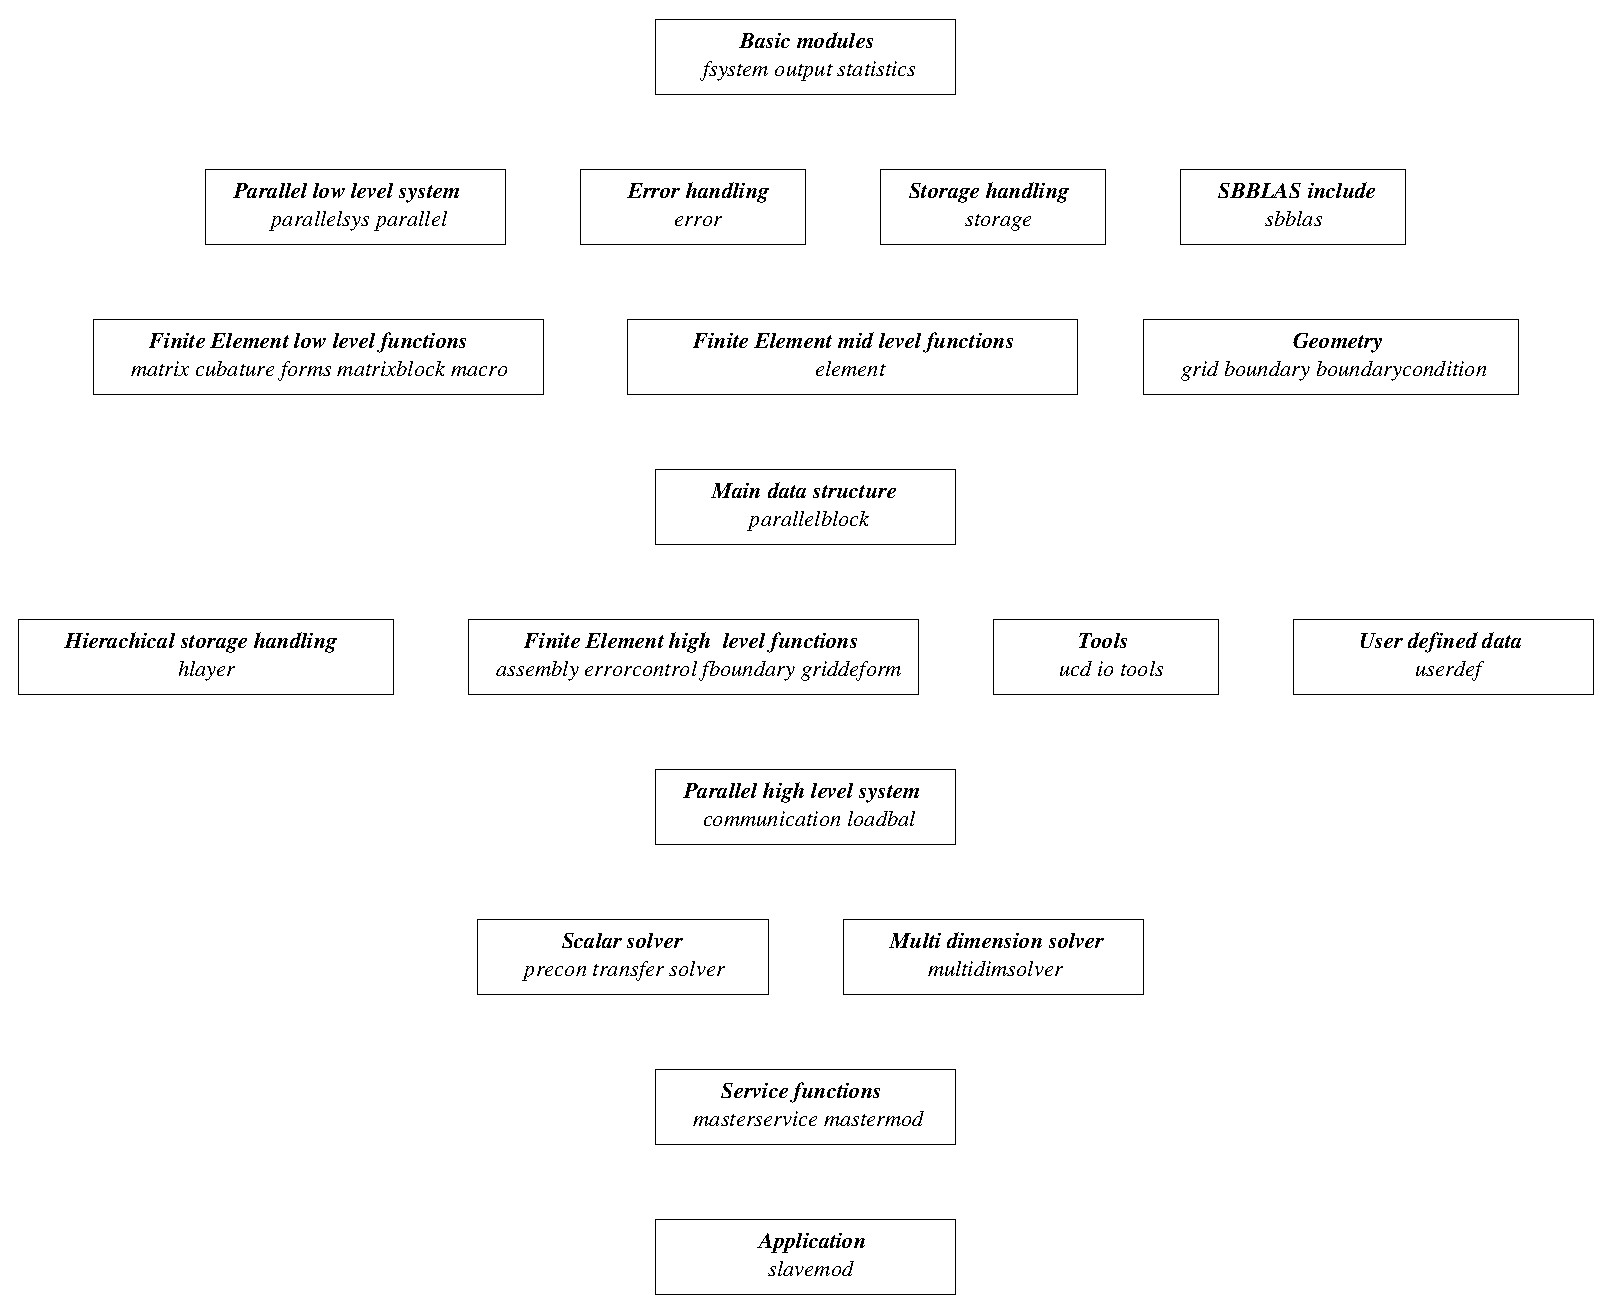
\includegraphics[scale=0.675]{../psfiles/modoverview.eps}
% \end{center}
% \caption{FEAST module overview}
% \label{modoverview}
% \end{figure}

This chapter gives a short overview of the structure of the
FEAT2 library and the purposes of the single modules. % Figure \ref{modoverview} shows the structure.



%\include{modules_overview_dynamic}
\include{modules_dynamic}

%\chapter{Module reference for application programmers}

\newpage


%\include{modules_description_dynamic}

% ---- Bibliography ----
%

\nocite{Turek1997c,Turek1998}
\bibliography{fbmathlit}

% ---- Index ----
%
\printindex

\end{document}
